\chapter{State-of-the-Art}
Crowd motion analysis deals with a combination of computer vision, Image processing and machine 
learning techniques. This section provides in depth knowledge of related work and state of the art 
techniques by explaining the recent and ground braking scientific papers in this field. More specifically 
the motivation introduction and the techniques used in these papers.
\section{Crowd analysis using optical flow}
The papers ~\cite{santoro2010crowd} ~\cite{rosandic2019crowd} gives a generic and very efficient way 
of tracking the crowd motion in the videos. As shown in the figure \ref{fig:opticaldataflow} below, the 
process of crowd tracking is done in 4 steps. 
\begin{figure}[tb]
	\center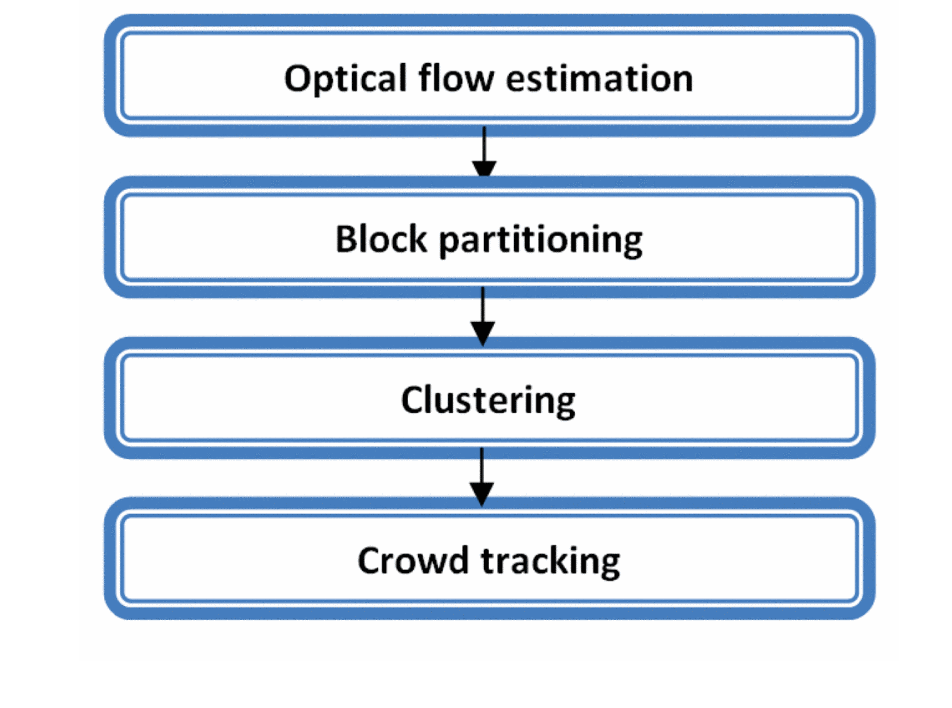
\includegraphics[width=0.6\textwidth]{Opticalflowdataflow.png}
	\caption{Data Flow Diagram}
	\label{fig:opticaldataflow}
\end{figure}
KLT feature tracker is used to do the optical flow estimation.KLT feature tracker is the combination of Shi-
Tomasi corner detection and the famous Lucas Kanade optical flow algorithm. Shi-Tomasi corner 
detection technique is used to identify the interesting corners of the frame. A section of surrounding 
pixels of these points are also added to the tracking. This step is followed by tracking the points in the 
consequent frames. The tracking is done with the help of Lucas Kanade algorithm. In addition to the 
change in the points, magnitude and the angle of the vector is also calculated at this point of time.

Now that all the vectors are derived from frame fk and fk+1, block partitioning is done on the whole 
frame. The frame is divided in to multiple blocks and the vectors in the specific blocks are clustered 
based on the angle and magnitude. This clustering is done with the help of DBSCAN algorithm. All the 
points which are considered to be one group are marked with single vector. Any person leaving the 
crowd or joining the crowd is considered as separate or single block accordingly. The result of this paper 
are shown in the figure \ref{fig:opticalflowresult}. The person behind the crowd is considered as separate 
group and the tracking is done multiple times to get the flow.
\begin{figure}[tb]
	\center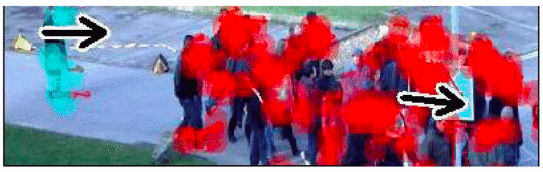
\includegraphics[width=0.6\textwidth]{opticalflowresult.png}
	\caption{Density based partitioning and crowd tracking}
	\label{fig:opticalflowresult}
\end{figure}

The paper ~\cite{cheriyadat2008detecting} is an interesting use of optical flow to detect the dominant 
motion in the crowded scenes. This paper suggests a combination of both Shi Tomasi corner detection 
algorithm and FAST corner detection to identify the  interesting points in the frame. Keeping track on 
interesting points in multiple frames, the trajectory is captured. New feature points are added in every 5 
frames to handle the load. The new feature points which are close to the old points are discarded. 
\begin{figure}[tb]
	\center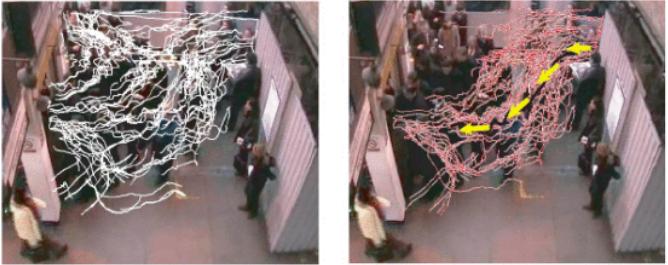
\includegraphics[width=0.6\textwidth]{dominantresult.png}
	\caption{Dominant motion detection results}
	\label{fig:dominantresult}
\end{figure}
By getting the trajectories of all the points, a new clustering framework Longest Common Subsequences 
(LCSS) is introduced. With the help of this framework, multiple trajectories are compared for the 
matching points and the dominant path is captured by clustering trajectories. The results of this model 
are shown in the figure \ref{fig:dominantresult}.

\section{Crowd counting}
Crowd counting is a difficult task and the accuracy of the proposed models depends on the scene. In 
case of large density of crowd, it is extremely hard to track the crowd for counting. Most recent paper 
~\cite{chen2020crowd} suggests that crowd counting can be done in 2 ways. The first is by using 
detection based models, where the crowd is being tracked with the help of body parts or the shape and 
the count is produced from the tracking model. The second is Regression based models, where the 
model predicts the number of the crowd with out tracking them. This model is based on developing a 
density map and estimating the count from the produced density map. A part from these 2 methods 
there is another method based on CNN, which also produced promising results. But, in the CNN 
models, there are cases where the system predicted various different objects as human heads causing 
a huge difference in the count.  ~\cite{chen2020crowd} deals with the combination of density based 
model and the CNN in order to fix the on going issue with the CNN models.

~\cite{5374413} is another interesting paper which can be grouped into the detection based models. In 
this paper, the writer creates a part-template tree with the human postures in different angles, poses 
and shapes. A hierarchical part-template matching algorithm is used to estimate human shapes and 
poses by matching local image. Multiple detectors are used to detect the multiple body shapes as 
shown in the figure \ref{fig:rmfmdcc}. The segmentation is done based on these multiple detectors. 
Background subtraction is used to evaluate the model and produced promising 
results.~\cite{chan2008privacy} can be grouped under the regression based model of counting crowds. 
This paper suggests the motion segmentation of the crowd clustered based on the direction. The count 
on the each direction is estimated using the Gaussian process. This model is explained in the figure 
\ref{fig:regcc}

\begin{figure}[tb]
	\center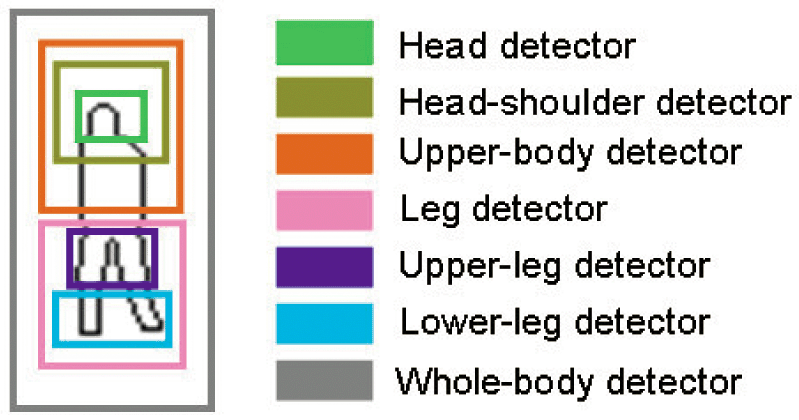
\includegraphics[width=0.6\textwidth]{Mfeaturemdetector.png}
	\caption{Multi Feature multi detector model}
	\label{fig:rmfmdcc}
\end{figure}

\begin{figure}[tb]
	\center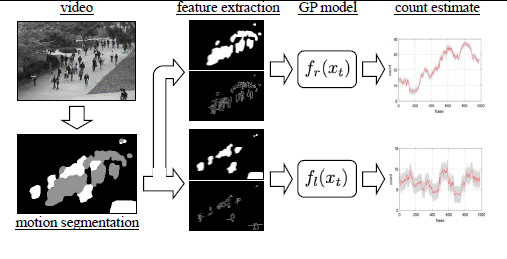
\includegraphics[width=0.6\textwidth]{RegressionCC.png}
	\caption{Regression Based crowd counting}
	\label{fig:regcc}
\end{figure}

\section{Motion detection and classification}
In order to understand the behaviour of the crowd, it is important to detect the motion and also classify 
them. For example to check if the vehicles are moving in the right path, people following the suggested 
path, person walking in restricted area etc. The crowd motion can be categorised into different groups 
based on the scene. If the scene is to identify the anomaly in the crowd motion for example in the traffic, 
the motion can be grouped into Lanes, Arcs, blocks. In case of entering or exiting enclosed buildings 
the motion can be Bottlenecks or Fountainheads. In case of violent protest, it can be categorised into 
converging or diverging. In all the cases, it is important to study the type of the motion in order to tackle 
the situation.

\begin{figure}[tb]
	\center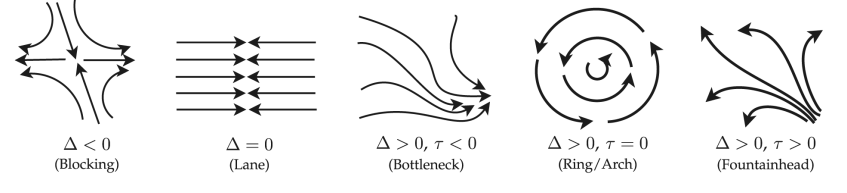
\includegraphics[width=0.6\textwidth]{stability.png}
	\caption{Types of motion based on the product and sum of eiganvalues}
	\label{fig:stability}
\end{figure}

~\cite{solmaz2012identifying} states that crowd motion can be categorised into 5 types: Lanes, Arcs, 
Bottlenecks, Fountainheads and Blocks. This paper suggests a model which can categorise the videos 
with out a training model. It used Particle advection to pick the interesting points in the frame and track 
these points as a spacio-temporal data. The motion is further produced in the equation using Taylor 
theorem. The stability of the motion is detected by calculating Jacobian Matrix. The eigenvalues of this 
matrix is used to classify the motion as shown in the figure \ref{fig:stability}.

\begin{figure}[tb]
	\center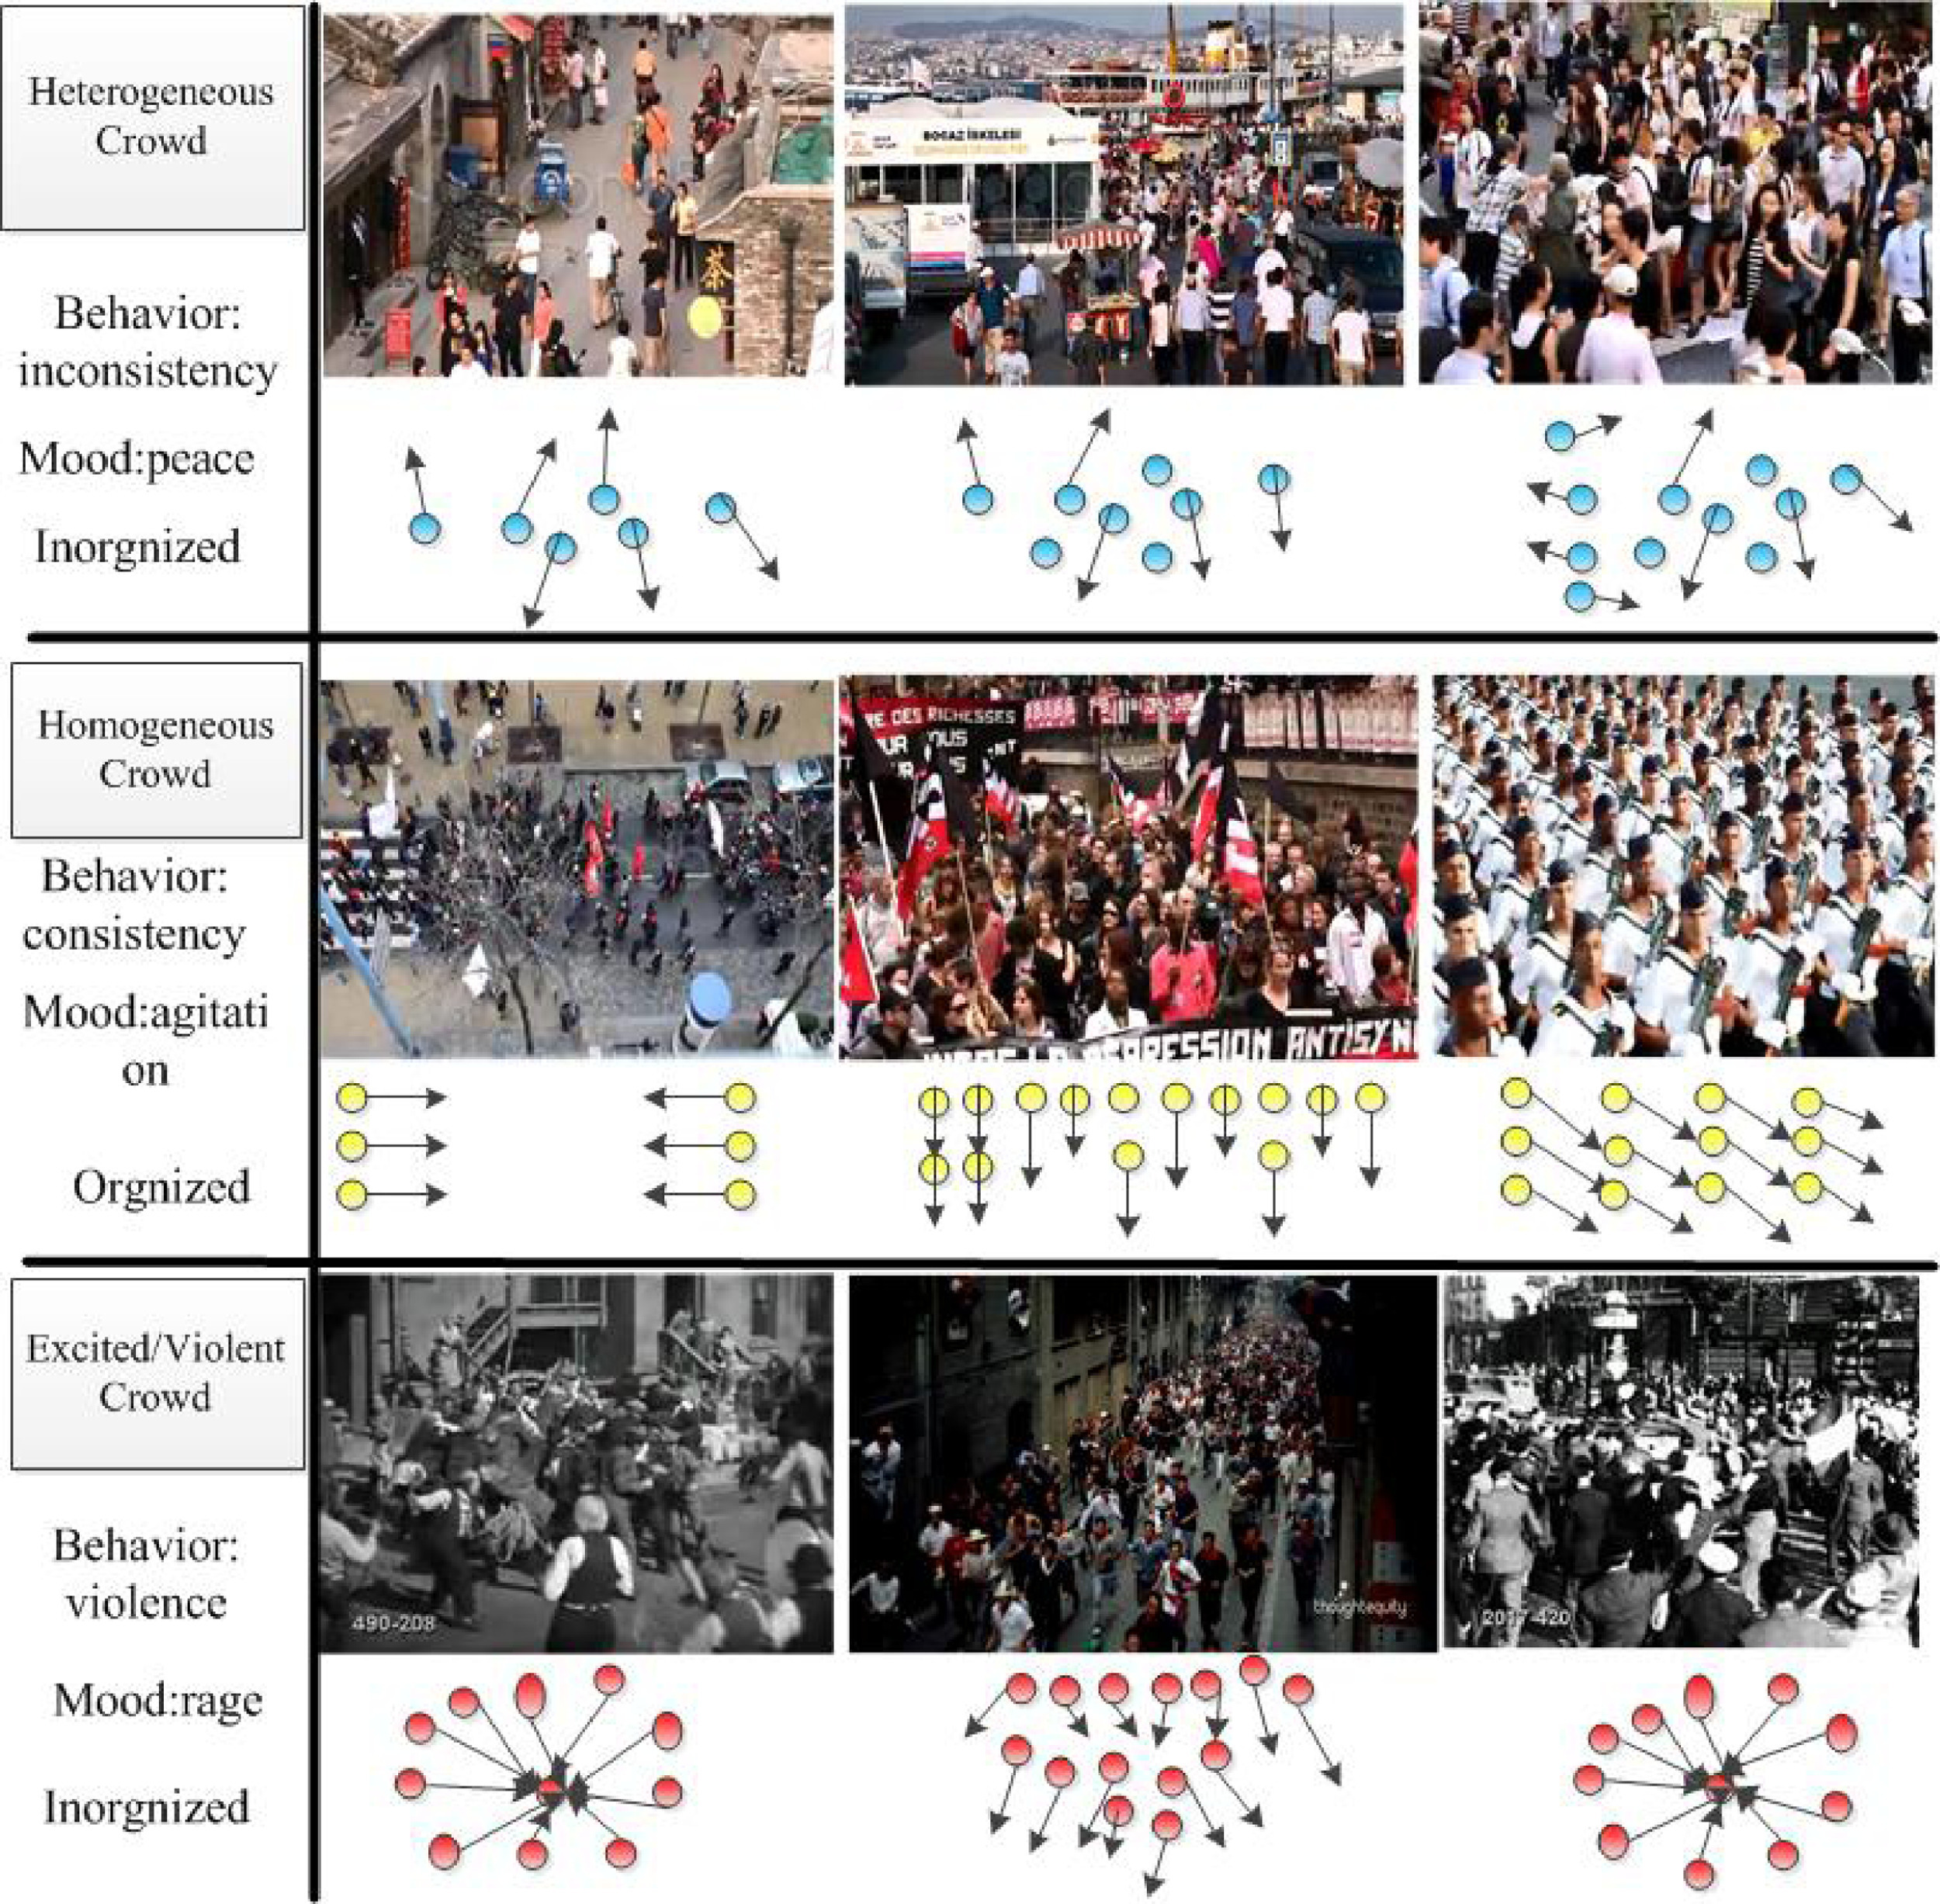
\includegraphics[width=0.6\textwidth]{deepnets.jpg}
	\caption{Crowd categorisation using 2 deep networks}
	\label{fig:2deep}
\end{figure}

Identifying the type of the crowd is key to understand the type of the action, scene of the incident and 
actions of the people. This paper ~\cite{wei2020very} categorise to crowd into 3 types based on a 
model called BMO model (Behaviour, Mood and Organisation model). This model is a rule based model 
which helps to detect the crowd motion to be grouped into Heterogenous, Homogenous and Violent 
crowds. To implement this model, they trained 2 very deep VGG networks and combined the FCN 
layers of both the networks to predict the type of the crowd. The inputs to these networks are the motion 
map and key frame. The results and the implementation of this model are shown in the figure 
\ref{fig:2deep}

\section{Anomaly detection in the crowd motion}
Another very interesting and key papers published are focused on the Anomaly detection. This type of papers focus on identifying unexpected behaviour in the frame. For example the paper ~\cite{bansod2020crowd} focuses on 3 types of anomalies, namely: Point Anomaly which points a single object in the frame. This can be an unexpected motion or sudden change in the magnitude of single object. The second type id the collective anomaly, where most of the objects in the frame experience sudden drift in the direction and velocity. This type of anomaly is usually found in the riots, explosions etc. The third type of anomaly is contextual anomaly which can be unexpected shaped object in the frame etc. The figure \ref{fig:anomaly} explains the different types of the anomalies clearly.

This paper implements the model with the footages from the stable surveillance cameras and techniques like background reduction. It also proposes a new way of gathering the features like direction, change in the points, distance etc. These features are further classified using k-means clustering and distance calculation to predict the motion to be expected or unexpected.

\begin{figure}[tb]
	\center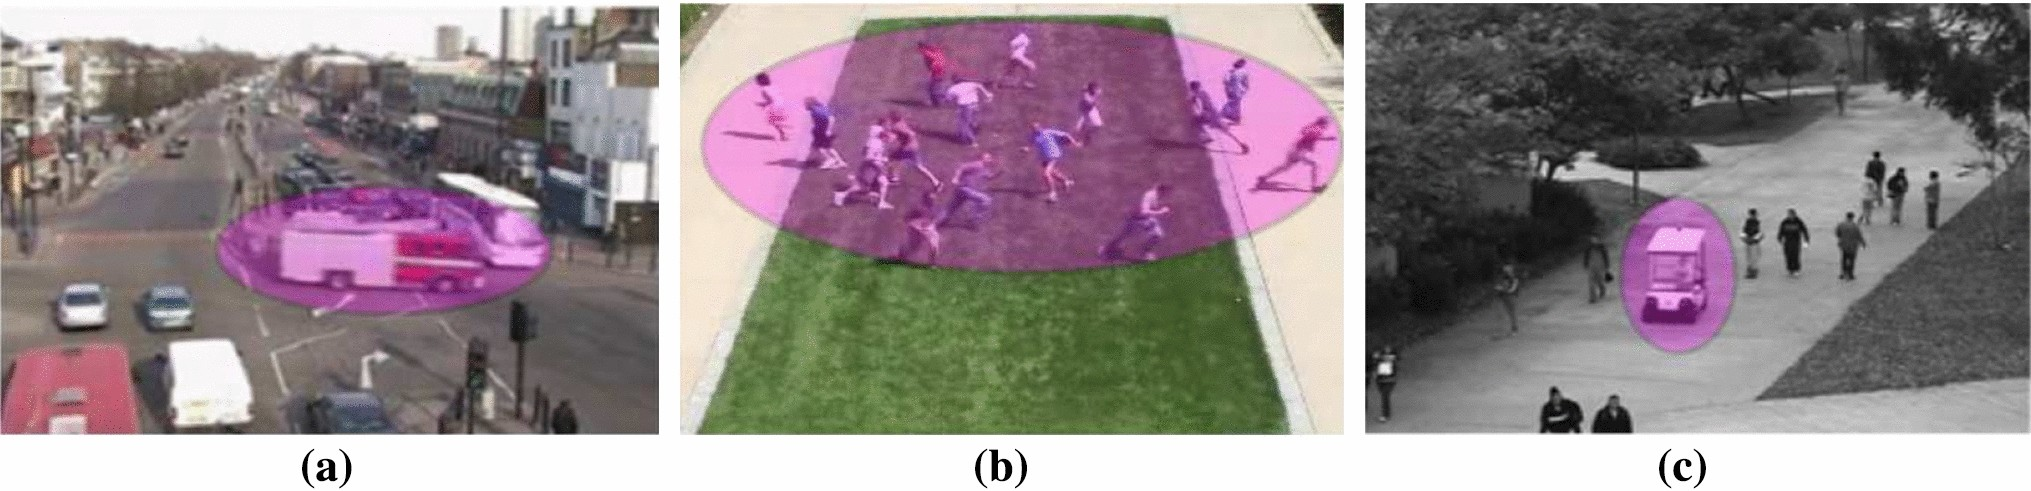
\includegraphics[width=0.6\textwidth]{anomaly.jpg}
	\caption{Types of anomalies}
	\label{fig:anomaly}
\end{figure}


 

 